\begin{surferPage}{El Doble Cono}
  En la introducción de esta galería, explicamos que una superficie
  se llama \emph{no--singular} o suave si no tiene picos (también conocidos
  como singularidades). Algunos ejemplos son las dos imágenes que encontramos
  a la izquierda, la esfera y el toro:
    \begin{center}
      \begin{tabular}{@{}c@{}c@{}c@{}c@{}}
        \begin{tabular}{@{}c}
          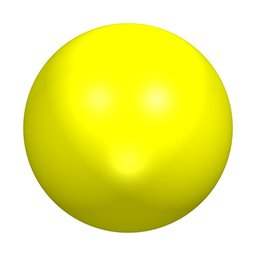
\includegraphics[width=1.4cm]{../../common/images/kugel}
        \end{tabular}
        &
        \begin{tabular}{@{}c}
          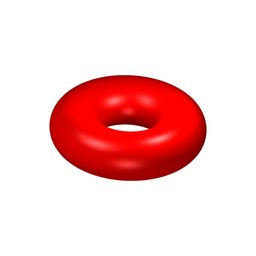
\includegraphics[width=1.4cm]{../../common/images/torus}
        \end{tabular}
        &
        \begin{tabular}{c@{}}
          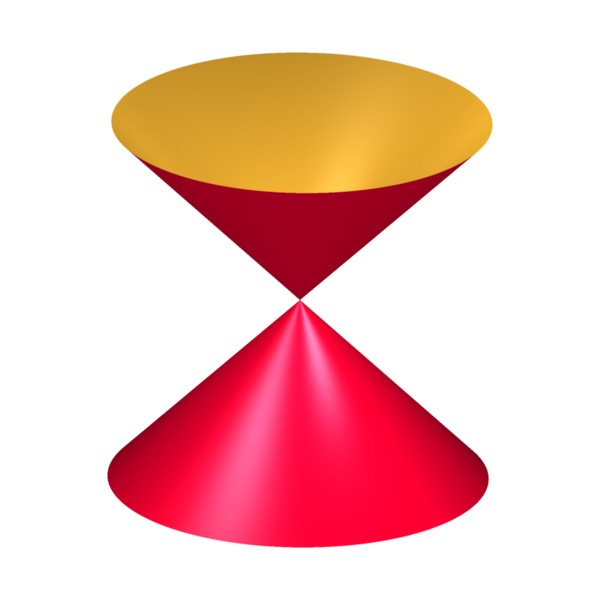
\includegraphics[width=1.4cm]{../../common/images/kegel}
        \end{tabular}
      \end{tabular}
    \end{center}
     El doble cono (la imagen de la derecha) es la superficie 
     más simple con alguna singularidad; puede describirse
     con una ecuación de grado $2$:
     \[x^2+y^2-z^2=0.\]
     Cuando cambiamos ligeramente la ecuación, reemplazando el $0$ por un pequeño
     valor $a\neq 0$, el doble cono se transforma en uno de dos tipos de hiperboloides,
     dependiendo del signo de $a$:
    \begin{center}
      \vspace{-0.2cm}
      \begin{tabular}{@{}c@{\ }c@{\ }c@{\ }c@{\ }c@{}}
        \begin{tabular}{@{}c@{}}
          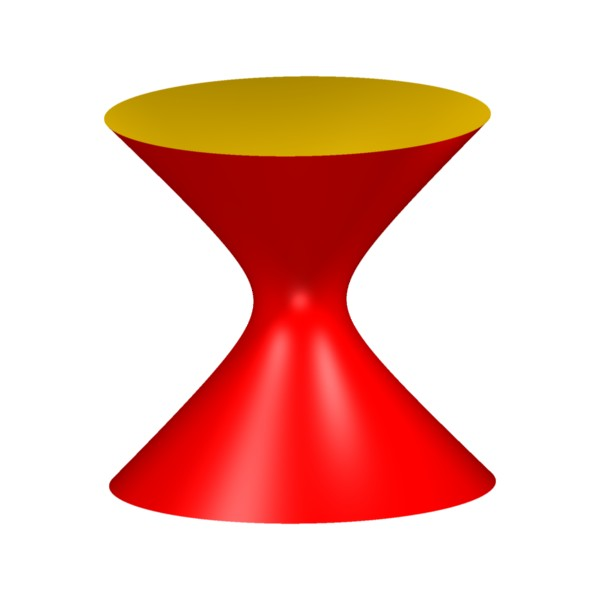
\includegraphics[width=1.2cm]{../../common/images/A1pm_2}
        \end{tabular}
        &
        $\leftarrow$
        &
        \begin{tabular}{@{}c@{}}
          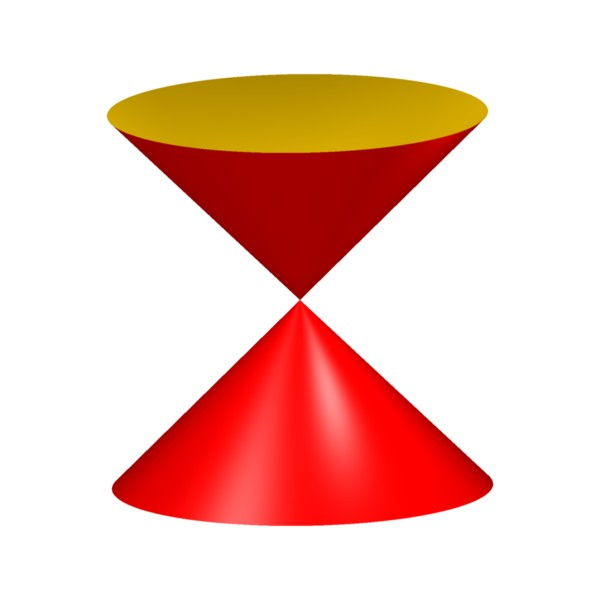
\includegraphics[width=1.2cm]{../../common/images/A1pm_1} 
        \end{tabular}
        &
        $\rightarrow$
        &
        \begin{tabular}{@{}c@{}}
          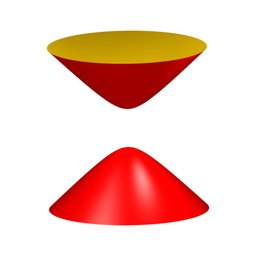
\includegraphics[width=1.2cm]{../../common/images/A1pm_0}
        \end{tabular}
      \end{tabular}
    \end{center}
   Una superficie de grado $2$ no puede tener más de una singularidad, es decir que $\mu(2)=1$.
\end{surferPage}
